\documentclass{llncs}
\usepackage{url}
\usepackage{proof}
\usepackage{amssymb}
\usepackage{stmaryrd}
\usepackage{listings}
\usepackage{graphicx}

\newcommand{\todo}[1]{\textbf{TODO: #1}}

%subcode-inline{bnf-inline} name langRev
%! swap+ = \mathit{swap}^+
%! swap* = \mathit{swap}^*
%! dagger =  ^{\dagger}
%! assocl+ = \mathit{assocl}^+
%! assocr+ = \mathit{assocr}^+
%! assocl* = \mathit{assocl}^*
%! assocr* = \mathit{assocr}^*
%! identr* = \mathit{uniti}
%! identl* = \mathit{unite}
%! dist = \mathit{distrib}
%! factor = \mathit{factor}
%! (o) = \fatsemi
%! (;) = \fatsemi
%! (*) = \times
%! (+) = +

%subcode-inline{bnf-inline} regex \{\{(((\}[^\}])|[^\}])*)\}\} name main include langRev
%! [^ = \ulcorner
%! ^] = \urcorner
%! [v = \llcorner
%! v] = \lrcorner
%! |-->* = \mapsto^{*}
%! |-->> = \mapsto_{\ggg}
%! |-->let = \mapsto_{let}
%! |--> = \mapsto
%! |- = \vdash
%! in = \!\!\in\!\!
%! <=> = \Longleftrightarrow
%! <-> = \leftrightarrow
%! ~> = \leadsto
%! ::= = ::=
%! /= = \neq
%! vi = v_i
%! di = d_i
%! si = s_i
%! sj = s_j
%! F = \texttt{F}
%! T = \texttt{T}
%! forall = \forall
%! exists = \exists
%! empty = \emptyset
%! eta = \eta
%! where = \textbf{where}
%! epsilon = \varepsilon
%! least = \phi
%! trace+ = trace
%! trace* = trace_{\times}
%! loop+ = loop_{+}
%! loop* = loop_{\times}
%! CatC = {\mathcal C}
%! CatA = {\mathcal A}
%! gamma = \gamma
%! {[ = \{
%! ]} = \}
%! elem = \in
%! dagger = ^\dagger
%! alpha = \alpha
%! beta = \beta
%! rho = \rho
%! @@ = \mu
%! @ = \,@\,
%! langRev = \Pi
%! langRevT = \Pi^{o}
%! langRevEE = \Pi^{\eta\epsilon}_{+}
%! bullet = \bullet
%! * = \times

\urldef{\mails}\path|{rpjames, sabry}@indiana.edu|

%%%%%%%%%%%%%%%%%%%%%%%%%%%%%%%%%%%%%%%%%%%%%%%%%%%%%%%%%%%%%%%%%%%%%%%%%%%%%

\begin{document}
\title{On the Construction of Isomorphic Interpreters} 
\titlerunning{On the construction of Isomorphic Interpreters} 
\author{Roshan P. James \and Amr Sabry}
\institute{School of Informatics and Computing, Indiana University\\
\mails}
\maketitle

%%%%%%%%%%%%%%%%%%%%%%%%%%%%%%%%%%%%%%%%%%%%%%%%%%%%%%%%%%%%%%%%%%%%%%%%%%%%%
\begin{abstract}
\end{abstract}

%%%%%%%%%%%%%%%%%%%%%%%%%%%%%%%%%%%%%%%%%%%%%%%%%%%%%%%%%%%%%%%%%%%%%%%%%%%%%
\section{Introduction} 


Previous work on {{langRevT}} \cite{rc2011,infeffects} studied its
properties and various constructions in it. However, for a
computational model, there has been little focus on actually writing
programs directly in {{langRevT}}. This paper aims to remedy that by
presenting a systematic technique of expressing logically reversible
small-step abstract machines in {{langRevT}}. This paper shows that
once we have a logically reversible machine in a notation of our
choice, expressing the machine as an isomorphic interpreter in
{{langRevT}} can be done systematically and does not present any
significant conceptual difficulties.

The constructions in this paper apply only to a class of interpreters
that can be represented by logically reversible small-step operational
semantics. While, in a formal sense, they are related to Abramsky's
``bi-orthogonal automata''\cite{abramsky2005structural}, we will try
to give them a more direct characterization purely in terms of logical
reversibility of the small-step semantics.

%%%%%%%%%%%%%%%%%%%%%%%%%%%%%%%%%%%%%%%%%%%%%%%%%%%%%%%%%%%%%%%%%%%%%%%%%%%%%
\section{Simple Bounded Iterator}
Consider definition for the following small-step abstract machine:

%subcode{bnf} include main
% Expressions, e = n
% Numbers, n, m = 0 | n + 1
%
% Machine states = <e, e>
% Start state = <n, 0>
% Stop State = <0, n>

Small-step Operational semantics:

%subcode{opsem} include main
% <n+1, m> |--> <n, m+1>

This machine start with a number {{n}} in the first position and at
each reduction step decrements the first number and increments the
second. It stops when the first number reaches 0, thereby taking
exactly {{n}} steps. While the machine does nothing interesting,
it useful to illustrate the general idea.

\begin{enumerate}
\item 
We can turn this abstract machine into a an isomorphic interpreter
implemented in {{langRevT}}, in a systematic way. To start with we
realize that the interpreter should implement the following map.

\begin{center}
  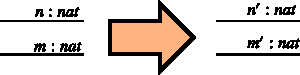
\includegraphics{diagrams/nat-nat1.pdf}
\end{center}

Now numbers can be implemented by the recursive type {{nat = @@x.1+x}}
in {{langRevT}}. This gives us the isomorphisms 

\begin{center}
  {{unfold : nat <-> 1 + nat : fold}}
\end{center}

We start by examining the first value. 

\begin{center}
  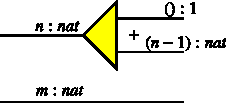
\includegraphics{diagrams/nat-nat2.pdf}
\end{center}

\item
The triangle denotes the {{unfold}} isomorphism, which works as
follows: If the number {{n}} is zero, the output is the top branch
which has type {{1}}. If the number was non-zero, the output is on the
bottom branch and has value {{n-1}}. 

Since the abstract machine increments second component, we know that
we need a {{fold}} on the second component to accomplish this. So we
can fill in the output part of the interpreter dually. 

\begin{center}
  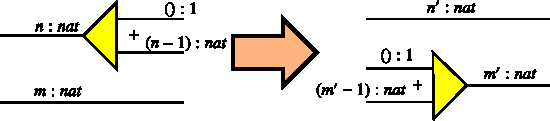
\includegraphics{diagrams/nat-nat3.pdf}
\end{center}

\item
Let us examine all the possible input states, by distributing on the
input. Dually let us do the same with the output, but this time also
be a little bit explicit about the swap operations required so the
right types are in place.

\begin{center}
  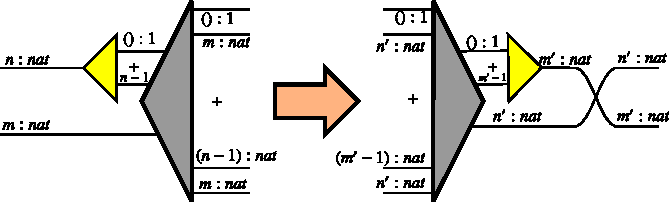
\includegraphics{diagrams/nat-nat4.pdf}
\end{center}

\item
The construction above already gives us some insight into how we can
implement our one reduction step. If we chose {{m = m'-1}} and we
chose {{n-1 =n'}} then we have essentially encoded the required
rewrite. Lets state this in words - the new value of {{n}}, namely
{{n'}}, is equal to {{n-1}}. And further - the new value of {{m}},
namely {{m'}}, is {{m+1}} (because {{m'-1=m}}). 

We can thus connect the lower branches with the appropriate
isomorphism to reflect this relationship. In this case the isomorphism
is just a swap of the two wires involved.

\begin{center}
  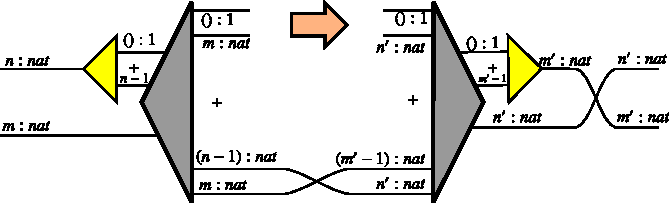
\includegraphics{diagrams/nat-nat5.pdf}
\end{center}

\item
We are a few steps away from an interpreter at this point and the
final steps rely on the answers to a few questions.

\begin{enumerate}
\item How do relate the outputs of the combinator to the inputs, such
  that the machine correctly takes multiple steps?

\item What do we do about the two inner branches? 

\end{enumerate}

The branch labeled {{((), m)}} looks like the stop state of the
machine. The branch label-led {{((), n')}} looks like the start state
of the program. To complete the interpreter, we flip our current
construction inside out.

\begin{center}
  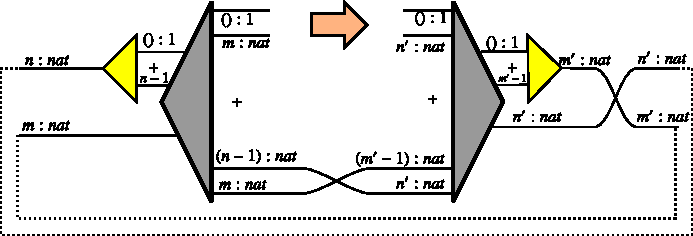
\includegraphics{diagrams/nat-nat6.pdf}
\end{center}

Which gives us

\begin{center}
  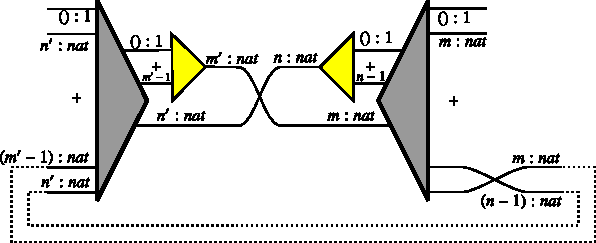
\includegraphics{diagrams/nat-nat7.pdf}
\end{center}

This basically completely our construction of the interpreter. We
basically need to use a {{trace}} to feedback related machine states
to related machine states.

\begin{center}
  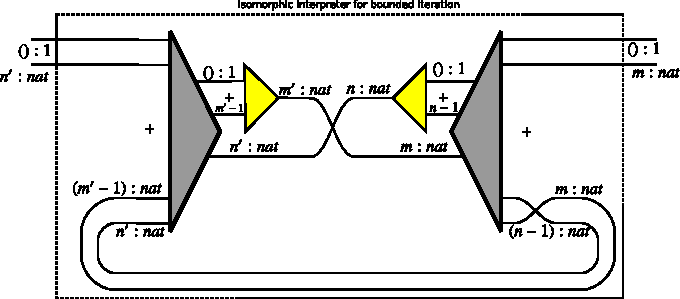
\includegraphics{diagrams/nat-nat8.pdf}
\end{center}

\end{enumerate}

%%%%%%%%%%%%%%%%%%%%%%%%%%%%%%%%%%%%%%%%%%%%%%%%%%%%%%%%%%%%%%%%%%%%%%%%%%%%%%%%%%%%%
\section{Abstracting out the Construction}

%%%%%%%%%%%%%%%%%%%%%%%%%%%%%%%%%%%%%%%%%%%%%%%%%%%%%%%%%%%%%%%%%%%%%%%%%%%%%%%%%%%%%
\subsection{What are the high level steps in the translation?}
\label{sec:steps}

TODO

\begin{enumerate}
\item Expand the input such that every input term that the LHS of the
  interpreter pattern matches on is exposed.

\item Expand the output such that every output term that it
  reconstructed by the interpreter is exposed.

\item Shuffle matching LHS term to matching RHS terms, inserting any
  appropriate mediating computations. In the previous example, this
  was only a swap operation.

\end{enumerate}

%%%%%%%%%%%%%%%%%%%%%%%%%%%%%%%%%%%%%%%%%%%%%%%%%%%%%%%%%%%%%%%%%%%%%%%%%%%%%%%%%%%%%
\subsection{What abstract machines can be turned into isomorphic interpreters?}

Logically reversible abstract machines with distinguishable start and
stop states can be converted into isomorphic interpreters in
{{langRevT}}.  To develop an understanding for what sorts of machines
these are, let us look at some examples.

Consider a machine with the following two reduction steps
 and . Can we create an
isomorphic interpreter for such a machine? We can't, because for any
given machine state, it is not obvious what reduction rule to
apply. We could reverse this machine if there was a clear
non-ambiguity in which machine rule was chosen.

Consider a machine, with the following rewrite rules
 and . Can we
create an isomorphic interpreter for this machine? It turns out we
can't because for any given output state  it is not
obvious which input state it came from - i.e. there are two
possibilities  or there is .

Consider a machine that has the addition rule 
where {{z}} is the sum of {{x}} and {{y}}. This machine again cannot
be turned into an isomorphic interpreter because the one reduction
rule does not have a logically inverse -- in other words, given a
{{z}}, we are unable to determine which {{x}} and {{y}} it originated
from.

If we had only the reduction relation , can we
construct an isomorphic interpreter? After all, every rewrite rule is
logically reversible. In fact, this is not possible because there is
no distinguished start state for such an interpreter and hence one
does not know when to stop during reverse execution.

\noindent
Conditions that must be satisfied for constructing a isomorphic
interpreter:

\begin{enumerate}

\item Distinguishable start and stop states. There may be more than one
  valid start state and more than one valid stop state.

\item Each valid machine state must match a unique reduction LHS. Each
  valid machine state must machine a unique reduction RHS.

\item Every reduction step must be computable (in {{langRevT}}) and
  must be logically reversible -- i.e. it must be possible to reduce
  from right to left.

\end{enumerate}


%%%%%%%%%%%%%%%%%%%%%%%%%%%%%%%%%%%%%%%%%%%%%%%%%%%%%%%%%%%%%%%%%%%%%%%%%%%%%%%%%%%%%
\section{Adder and Multiplier}

\subsection{Logically Reversible Adder}

%subcode{bnf} include main
% Expressions, e = n
% Numbers, n, m,p = 0 | n + 1
%
% Machine states = <e, e, e>
% Start state = <n, p, 0>
% Stop State = <0, p', m>

Small-step Operational semantics:

%subcode{opsem} include main
% <n+1, p, m> |--> <n, p+1, m+1>

This is an ostensibly useful machine in the sense that it computes the
sum of its two inputs.  This construction proceeds exactly like the
previous one till we have the following situation:

\begin{center}
  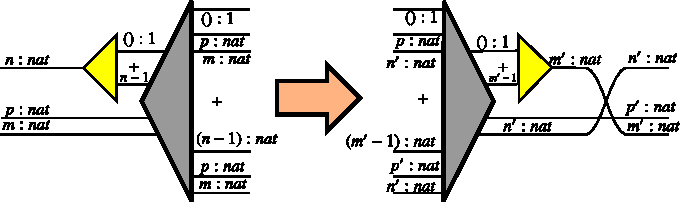
\includegraphics{diagrams/adder1.pdf}
\end{center}

The equalities we would like to express at this point are {{n-1=n'}},
{{m=m'-1}} and that {{p+1=p'}}. Fortunately {{langRevT}} provides the
{{add1: nat <-> nat}} combinator and so we could just use that to
mediate between {{p}} and {{p'}}. This is one solution and this gives
us:

\begin{center}
  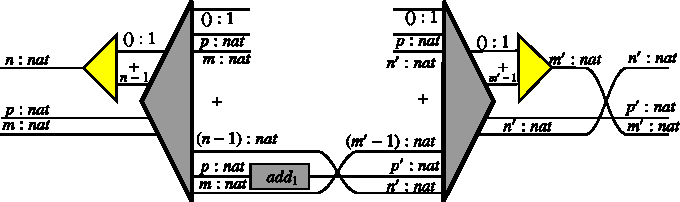
\includegraphics{diagrams/adder2.pdf}
\end{center}

This can be inverted as before, to give us an interpreter. While this
is a correct implementation of the small-step semantics, it is
somewhat unsatisfying for the reason that it does not see very
systematic. After all we chose to use an {{add1}} for {{p}} -- why
didn't we do the same for {{m}}? More importantly, the fact that we
chose used {{add1}} is also hiding something -- namely that {{add1}}
is a partial isomorphism. Its inverse is not defined when applied to
{{0}} i.e. it will go into an infinite loop. 

In a sense this implicit asymmetry of the abstract machine was being
hidden by the {{add1}} operation. So instead of choosing to use
{{add1}} let us chose to expand out {{p'}}, as recommended by step 2
in section \ref{sec:steps}. This gives us the following: 


\begin{center}
\scalebox{0.9}{
  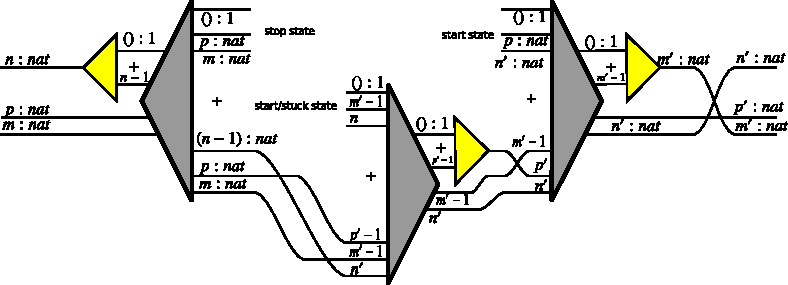
\includegraphics{diagrams/adder3.pdf}
}
\end{center}

We can very that the connected wires do indeed give us the desired
equalities between the inputs and outputs. Also we recognize our
expected start state and expected stop state. What is the dangling
state?

The dangling state was what has hidden by the use of {{add1}} and
denotes the fact that the abstract machine did not define any valid
backward reduction for the following valid machine state
. To take a backward step, both {{m}} and {{p}} have to
be simultaneously decremented and this is not possible if {{p}} is
{{0}}.  At this point we have two choices:

\begin{enumerate}
\item We can hide the use the combinator {{omega : b <-> 0}}
  expressible in {{langRevT}}. This combinator is basically an
  infinite loop on all inputs and hence would allow us to entirely
  discard one possible branch. In other words, we are explicitly
  admitting that our machine is undefined on some inputs.

\item We can admit that there are two possible start states to this
  abstract machine  and . One of this is an
  artifact of the fact that backward execution encounters stuck
  states. Dually, if there were stuck states for forward execution,
  they would be reflected in the fact that there were multiple stop
  states -- only one of which denotes a desirable or correct execution
  of the machine.

\end{enumerate}

As we did before, we flip inside out the construction so far and
apply {{trace}} to get the isomorphic interpreter:

\begin{center}
\scalebox{0.9}{
  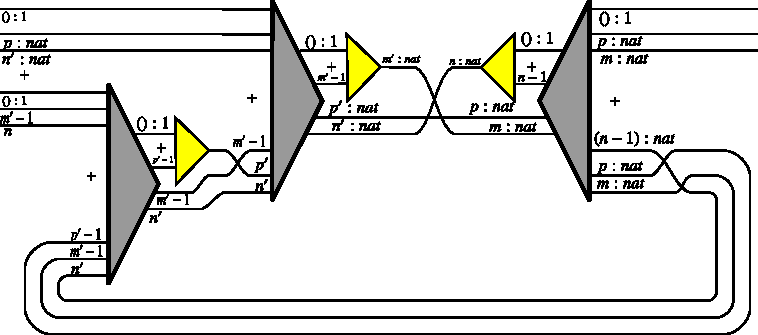
\includegraphics{diagrams/adder4.pdf}
}
\end{center}

%%%%%%%%%%%%%%%%%%%%%%%%%%%%%%%%%%%%%%%%%%%%%%%%%%%%%%%%%%%%%%%%%%%%%%%%%%%%%%%%%%%%%
\subsection{Logically Reversible Multiplier}


%%%%%%%%%%%%%%%%%%%%%%%%%%%%%%%%%%%%%%%%%%%%%%%%%%%%%%%%%%%%%%%%%%%%%%%%%%%%%%%%%%%%%
\section{Tree Traversal}

Let us take the ideas developed so far and apply them to developing a
tree traversal interpreter. We define a typical binary tree, one that
has numbers as leaf values and also define a notion of tree
contexts. The tree contexts serve to track which subtree is currently
being explored and are similar to tree zippers CITE.

%subcode{bnf} include main
% Tree, t = L n | N t t
% Tree Contexts, c = Lft c t | Rgt t c | []
%
% Machine states = <t, c> | {[c, t]}
% Start state = <t, []>
% Stop State = {[[], t]}

We define an abstract machine whose task is to traverse a given tree
and increment every leaf value. Small-step Operational semantics:

%subcode{opsem} include main
% <L n, c> &|-->& {[c, L (n+1)]}
% <N t1 t2, c> &|-->& <t1, Lft c t2>
% {[Lft c t2, t1]} &|-->& <t2, Rgt t1 c>
% {[Rgt t1 c, t2]} &|-->& {[N t1 t2, c]}

The machine here is a little richer than the ones dealt with
previously. In particular, we have a two types of machine states --
 and {{ {[t, c]} }}. One of these corresponds to walkking
down a tree, building up the context in the process. The other
corresponds to reconstructing the tree from the context and also
switching focus to any unexplored subtrees in the process. There are
also two syntactic categories to deal with -- trees and tree context
-- where previously we only had numbers. The {{fold}} and {{unfold}}
isomorphisms that we need for trees and tree contexts are:

%subcode{bnf} include main
%! columnStyle = rrcll
% unfold_t :& ~~~~t &<->& n + t * t &: fold_t
% unfold_c :& c &<->& 1 + c * t + t * c ~~~~~~&: fold_c

However we will see that the previously developed systematic approach
developing {{langRevT}} interpreters carries over to this abstract
machine as well.  As the first step, we quickly check that the
abstract machine however has disstinguished start and stop states, has
no ambiguities in reduction and that each reduction step is logically
reversible.

\subsection{New Notation}

Before we start on the actual construction, let us introduce a
syntactic convenience. In the past interpreter we explicitely drew out
every {{fold}} and {{unfold}} followed/preceded immediately by any
required swaps and then a {{distribute}} or {{factor}}. In this
presentation we will combine all of these into one construct which we
will draw as a thin vertical rectangle. Also we will introduce the
convention that the component that is being expanded or collapsed will
be marked by using {{[^ ^]}} and the components that are being
generated will be marked by {{[v v]}}. 

\begin{center}
\scalebox{1.0}{
  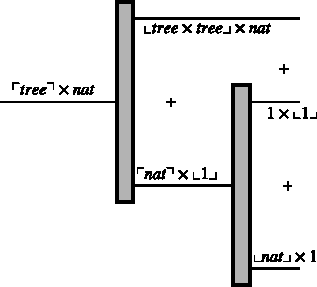
\includegraphics{diagrams/syntax1.pdf}
}
\end{center}

The above shows the expansion of a {{tree*nat}} type. First the
{{tree}} component is expanded and in one of the generated branches
the {{nat}} component is expanded.

%%%%%%%%%%%%%%%%%%%%%%%%%%%%%%%%%%%%%%%%%%%%%%%%%%%%%%%%%%%%%%%%%%%%%%%%%%%%%%%%%%%%%
\subsection{Isomorphic Interpreter}

The first step to developing teh isomorphic interpreter is to
recognize that the two possible kinds of machine states simply hide an
implicit {{bool}}. We make this explicit. 

%subcode{opsem} include main
% columnStyle = rclr
% <T, L n, c> &|-->& <F, L (n+1), c> &~~~~~ rule 1
% <T, N t1 t2, c> &|-->& <T, t1, Lft c t2> & rule 2 
% <F, t1, Lft c t2> &|-->& <T, t2, Rgt t1 c> & rule 3
% <F, t2, Rgt t1 c> &|-->& <F, c, N t1 t2> & rule 4

And so machine states have the form:

%subcode{bnf} include main
% Machine states = <bool, t, c>
% Start state = <T, t, []>
% Stop state =  <F, t, []>


And we start examining the machine components as before:

\begin{center}
\scalebox{0.9}{
  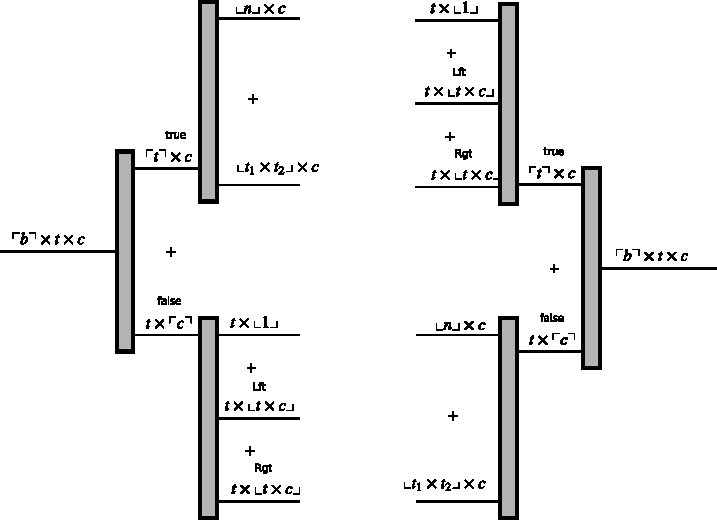
\includegraphics{diagrams/tree1.pdf}
}
\end{center}

On the LHS, for {{T}} states, we have expanded the tree component and
for {{F}} states we have expanded the tree contexts. Similarly we have
done the opposite on the RHS side exactly matching up what the
abstract machine does. One thing to note is that we dropped the {{1}}
introduced by expanding the {{bool}} and instead just labelled the
{{true}} and {{false}} branches.

We are ready to start connecting the machine states corresponding to
the reductions that we would like. 

\begin{enumerate}

\item 
When we encounter a leaf we would like to increment its value and move
to the corresponding {{F}} machine state. For the sake of simplicity
in this interpreter we won't be concerned with exposing stuck states
on reverse execution caused by {{sub1 0}}. So we are free to use the
{{add1}} combinator.

\item
For all the other reduction rules, it is a straight forward mapping of
related states following the reduction rules. 

\end{enumerate}

The required reduction rules have been labeled on the construction
belong. We have also included subscripts on the various {{t}}s to
indicate any swaps that may need to be inserted.

\begin{center}
\scalebox{0.9}{
  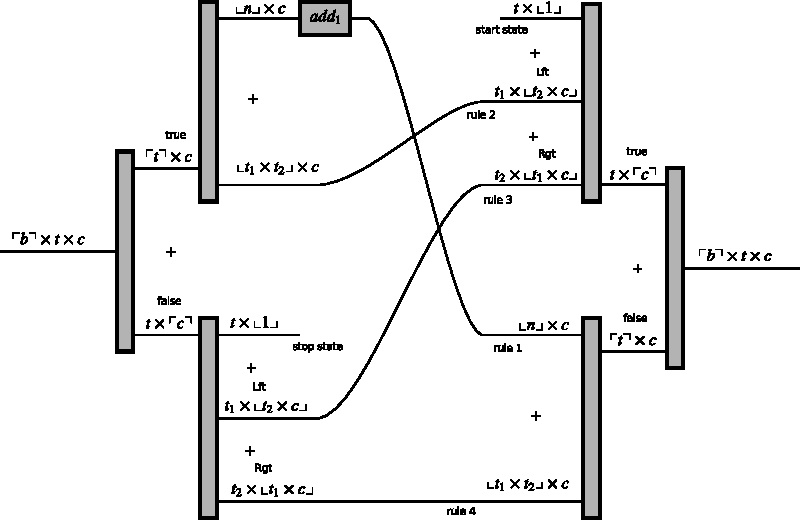
\includegraphics{diagrams/tree2.pdf}
}
\end{center}

This essentially completes the construction of the (partially)
isomorphic tree-traversal interpreter. (Partially because of the
implicit non-termination introduced by the {{add1}}).

%%%%%%%%%%%%%%%%%%%%%%%%%%%%%%%%%%%%%%%%%%%%%%%%%%%%%%%%%%%%%%%%%%%%%%%%%%%%%%%%%%%%%
\section{A {{langRev}} Interpreter}

%subcode{bnf} include main
% Combinators, c = iso | c (;) c | c (*) c | c (+) c
% Combinator Contexts, cc = [] | Fst cc c | Snd c cc 
%                  &|& LeftTimes cc c v | RightTimes c v cc 
%                  &|& LeftPlus cc c | RightPlus c cc 
% Values, v = () | (v, v) | L v | R v
%
% Machine states = <c, v, cc> | {[c, v, cc]}
% Start state = <c, v, []> 
% Stop State = {[c, v, []]}



%subcode{opsem} include main
%! columnStyle = rclr
% <iso, v, cc> &|-->& {[iso, iso(v), cc]} &~~~~~~~~~~~~ rule 1
% <c1(;)c2, v, cc> &|-->& <c1, v, Fst cc c2> &~~~~~~~~~~~~ rule 2
% {[c1, v, Fst cc c2]} &|-->& <c2, v, Snd c1 cc> &~~~~~~~~~~~~ rule 3
% {[c2, v, Snd c1 cc]} &|-->& {[ c1(;)c2, v, cc ]} &~~~~~~~~~~~~ rule 4
% <c1(+)c2, L v, cc> &|-->& <c1, v, LeftPlus cc c2> &~~~~~~~~~~~~ rule 5
% {[ c1, v, LeftPlus cc c2 ]} &|-->& {[c1 (+) c2, L v, cc ]} &~~~~~~~~~~~~ rule 6
% <c1(+)c2, R v, cc> &|-->& <c2, v, RightPlus c1 cc> &~~~~~~~~~~~~ rule 7
% {[ c2, v, RightPlus c1 cc ]} &|-->& {[c1 (+) c2, R v, cc ]} &~~~~~~~~~~~~ rule 8
% <c1(*)c2, (v1, v2), cc> &|-->& <c1, v1, LeftTimes cc c2 v2> &~~~~~~~~~~~~ rule 9
% {[ c1, v1, LeftTimes cc c2 v2 ]} &|-->& <c2, v2, RightTimes c1 v1 cc> &~~~~~~~~~~~~ rule 10
% {[ c2, v2, RightTimes c1 v1 cc ]} &|-->& {[ c1 (*) c2, (v1, v2), cc ]} &~~~~~~~~~~~~ rule 11


\begin{center}
\scalebox{0.9}{
  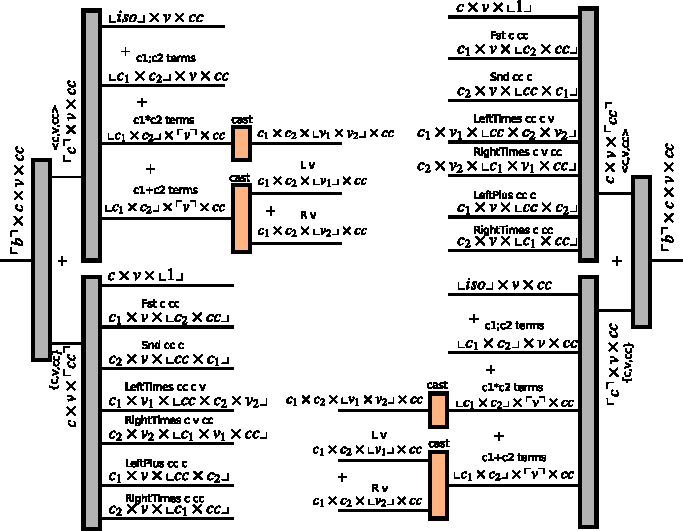
\includegraphics{diagrams/pi1.pdf}
}
\end{center}

\begin{center}
\scalebox{0.9}{
  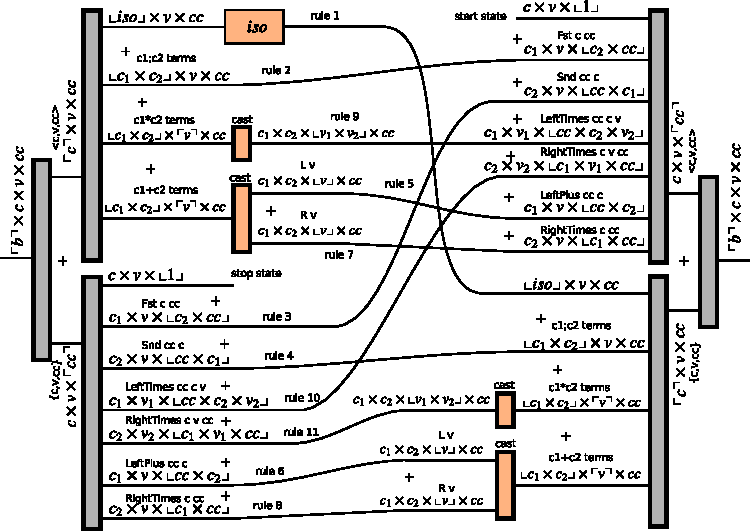
\includegraphics{diagrams/pi2.pdf}
}
\end{center}



TODO : The real difficulty with this interpreter is to argue why it is
not full of undefined states. For instance, why the machines will
never reach stuck states such as .  The right way
out of that is to make the type system of the abstract machine rich
enough that the structure of the abstract automatically rules out this
sort of thing. 

%subcode{bnf} include main
% Combinators, c(t1<->t2) = 
%             &|& c(t<->t) = iso 
%             &|& c(t1<->t2) = c(t1<->t3) (;) c(t3<->t2) 
%             &|& c(t1*t2<->t3*t4) = c(t1<->t3) (*) c(t2<->t4) 
%             &|& c(t1+t2<->t3+t4) = c(t1<->t3) (+) c(t2<->t4)
%
% Combinator Contexts, cc = [] | Fst cc c | Snd c cc 
%                  &|& LeftTimes cc c v | RightTimes c v cc 
%                  &|& LeftPlus cc c | RightPlus c cc 
%
% Type Indexed Values, v(t) =
%  &|& v(1) = () 
%  &|& v(t1*t2) = (v(t1), v(t2)) 
%  &|& v(t1+t2) = L v(t1) | R v(t2)
%
% Machine states = <c, v, cc> | {[c, v, cc]}
% Start state = <c, v, []> 
% Stop State = {[c, v, []]}


However this begs the question - does {{langRevT}} need all these GADT
types to reason about all these things? Something to think about. If
we do, then thereare two ways out 

(1) add GADTs to {{langRevT}} and keep the structure of things
simple. They can always be added opaquely for any given types -- we
only need to add the proper fold/unflod morphisms for those types
(maybe).

(2) compile down to {{langRevT}} as it is. In this case, {{langRevT}}
is indeed a relatively less typed language than the source language
and will hence have to treat as stuck-states the non-type correct
machine states. We could apply omega to them and make them vanish --
for example. This is similar to the handling of the {{sub1}} in the
previous example. 

%%%%%%%%%%%%%%%%%%%%%%%%%%%%%%%%%%%%%%%%%%%%%%%%%%%%%%%%%%%%%%%%%%%%%%%%
\section{A {{langRevEE}} interpreter}

\begin{center}
\scalebox{0.9}{
  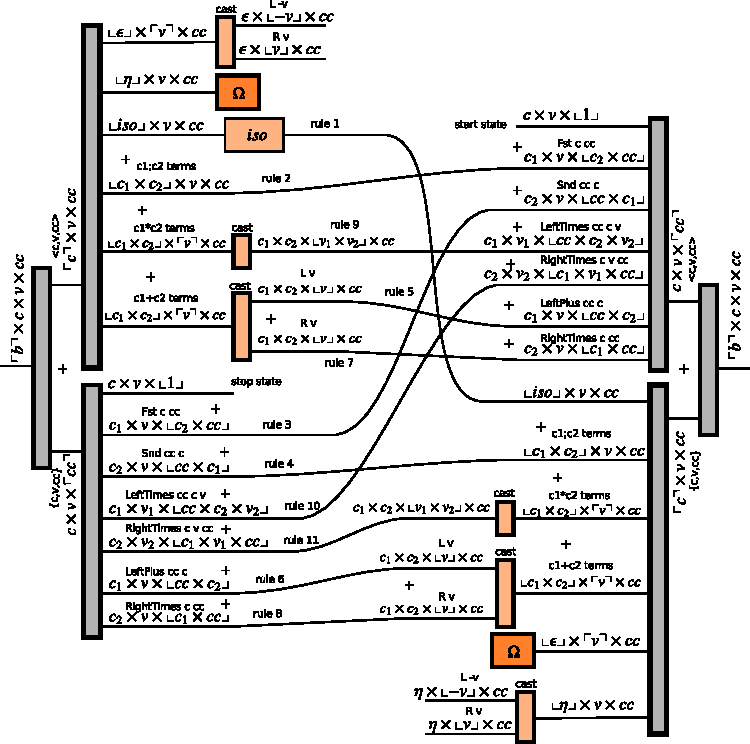
\includegraphics{diagrams/piee1.pdf}
}
\end{center}

Let us summarize it as follows.

\begin{center}
\scalebox{1.0}{
  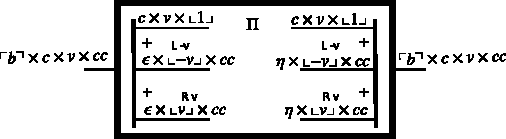
\includegraphics{diagrams/piee2.pdf}
}
\end{center}

Adding backward execution using the adjoint.

\begin{center}
\scalebox{1.0}{
  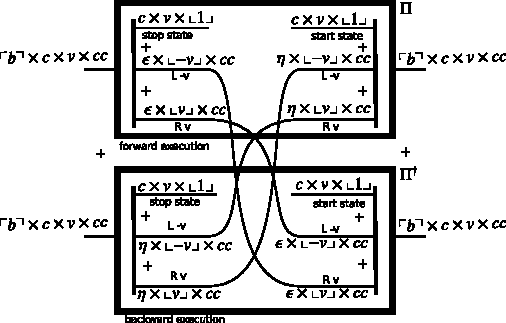
\includegraphics{diagrams/piee3.pdf}
}
\end{center}


\bibliographystyle{splncs03} 
\bibliography{cites}
\end{document}

